% !TEX root = omar-thesis-proposal.tex
\vspace{-25pt}
\section{Motivation}\label{motivation}
\begin{quote}\textit{The recent development of programming languages suggests that the simul\-taneous achievement of simplicity 
and generality in language design is a serious unsolved 
problem.} -- John Reynolds, 1970 \cite{Reynolds70}\end{quote}
%%One might exp ``generality''
%Designing a general-purpose programming language along with its supporting tools (collectively, a \emph{programming system}) has long stood as a grand challenge in computing. 
Achieving both simplicity and generality in the design of a programming language and its associated tools (collectively, a \emph{programming system}) requires organizing around a small number of mechanisms that support the expression of many others   as libraries. % In such a system, new dialects and revisions of the system would rarely be necessary. %Indeed, a preponderence of new dialects is clear evidence against claims of generality.  %Not all useful abstractions can be  realized, when considered comprehensively, as libraries.% The problem of achieving both simplicity and generality simultaneously with a single system remains unsolved. 
Much progress has been made in the decades since Reynolds' statement above, but  across all language lineages,  new language and tool \emph{dialects} remain common vehicles for new ideas, both in research and practice. This suggests that library-based mechanisms are still not general enough to encompass all desirable modes of expression. %Library implementations are not yet satisfying.

We will consider the broad class of situations where providers need to introduce new concrete syntax, type system fragments, or editor services into a system to realize an idea. %, encouraged  historically  by the availability of tools like compiler generators and,  more recently, language workbenches \cite{workbenches} and DSL frameworks \cite{dsl}. Unfortunately, taking this approach makes it substantially more difficult for clients to import high-level abstractions orthogonally. 
Equipping the system with \emph{extension mechanisms} that decentralize control over these features would  decrease the need for dialects, but this must done with care, because giving away too much control could also weaken the metatheory of the system. For example, were extensions allowed to arbitrarily modify the type system of the language, there would be immediate questions about {type safety}. Moreover, extension   mechanisms must come with \emph{modular reasoning principles} for it to be practical for library clients to rely upon them. Having to resolve conflicts between extensions or reestablish correctness properties of a program whenever a new extension is imported is unacceptably complex. %It can also make it more difficult to define new sorts of tools for working with the language because they cannot rely on there being a fixed abstract syntax (the canonical \emph{expression problem}). For programmers, 
%It can make it difficult to understand and reason about the type of an unfamiliar term, a critical facet of program comprehension (the \emph{typing discipline problem}).

In this thesis, we will design extension mechanisms that handle these issues, permitting library-based expression of features that today would need to be built into a system by its central designers. More specifically, we show how to delegate control over certain aspects of the concrete syntax, external type system and editor services to \emph{static functions}, i.e. user-defined functions written in a \emph{static language}. By layering these mechanisms over a fixed typed internal language, constraining the static language appropriately and validating the code it generates, we will retain key  metatheoretic properties and arrive at powerful modular reasoning principles. %By associating these static functions with type constructors, forming \emph{active type constructors},  we will further show how they can enjoy a usage profile essentially identical to that of built in features. % while maintaining key metatheoretic properties and modular reasoning principles. % By keeping the abstract syntax fixed and layering these mechanisms atop a fixed typed internal language (essentially lifting the first stages of compilation into the language), we avoid most aspects of the expression problem. %By delegating control to user-defined functions provided alongside user-defined type constructors (forming \emph{active type constructors}), we can give library providers substantially more control over these features of the system. 
%We structure each mechanism that we introduce as a \emph{bidirectional type system} combined with an  \emph{elaboration semantics} targeting a fixed typed internal language. 
%By constraining these functions and enforcing critical abstraction barriers between extensions, we will ensure key metatheoretic properties of the language and system components and guarantee that extensions can be reasoned about modularly. %We call user-defined types that introduce new features into the system in this way \emph{active types}.  % also highly expressive.
%But taking a \emph{language-internal approach} to implementing a feature is the most practical. If a feature can be realized by creatively using existing language constructs and distributed as a library, clients face fewer barriers to adoption because it is easy to integrate library-based features into existing projects gradually and granularly and they leverage well-understood and well-developed mechanisms.
% But taking this approach is often \emph{not} possible today %We call designs \emph{monolithic programming systems}.

%To realize a new abstraction or system behavior, such experts can consider either a \emph{language-internal approach}, where they work within an existing language and distribute their solutions as libraries, or a \emph{language-external approach}, where they create a new, distinct programming system (often centered around what has come to be called a new \emph{domain-specific language} \cite{dsl}) or extend an existing system by some mechanism that is not part of the language itself, such as an extension mechanism supported by a {particular} compiler, editor or other tool.

\subsection{Motivating Examples}\label{sec:examples}
To make the use cases we seek to address more concrete, let us begin with a few simple examples that we will return to throughout this work.

\subsubsection{Example 1: Regular Expressions}\label{sec:regex}
\emph{Regular expressions} are commonly used to capture patterns in strings (e.g. motifs in DNA sequences) \cite{Thompson:1968:PTR:363347.363387}. Programmers who work with regular expressions would benefit from features like these:

\begin{enumerate}
\item \textbf{Concrete syntax for pattern literals}. An ideal syntax would permit programmers to express patterns in the concise, conventional manner. For example, consider a bioinformatics  application: the BisI restriction enzyme cuts DNA when it sees the motif \texttt{GC\textit{N}GC}, where \texttt{\textit{N}} is any base. We would want to express such patterns with syntax like this, using curly braces to splice one pattern into another and parentheses to delimit captured groups:
\begin{lstlisting}[numbers=none]
let N : Pattern = <SURLA|T|G|CEURL>
let BisI : Pattern = <SURLGC({EURLNSURL})GCEURL>\end{lstlisting}
%The cognitive load of reading and writing patterns is low and patterns are parsed once at compile-time. 
Malformed patterns would ideally result in intelligible \emph{compile-time} parse errors.
\item A \textbf{static semantics} that ensures that key invariants related to regular expressions are statically maintained. For example, 
	\begin{enumerate}
	\item At minimum, we would want that only patterns, or properly escaped strings, are spliced into a pattern literal like that above, to avoid splicing errors and injection attacks \cite{owasp2013, Bravenboer:2007:PIA:1289971.1289975}. For example,
\begin{lstlisting}[numbers=none]
let fourChars : string = '\d\d'
let twoDigits : Pattern = <SURL\d\dEURL>
let p : Pattern = <SURL{EURLfourCharsSURL}-{EURLtwoDigitsSURL}EURL>
\end{lstlisting}
    should either be ill-typed because \lstinline{fourChars} is not a pattern, or be equivalent to the following:
\begin{lstlisting}[numbers=none]
let p : Pattern = <SURL\\d\\d-\d\dEURL>
\end{lstlisting}
    It should \emph{not} treat the string incorrectly as a pattern:
\begin{lstlisting}[numbers=none]
let p : Pattern = <SURL\d\d-\d\dEURL> (* injection attack vector! *)
\end{lstlisting}
	\item A more advanced semantics might ensure that out-of-bounds backreferences to a captured group do not occur \cite{spishak2012type}. For example, we would want \verb|BisI|, above, to have the more precise type \verb|Pattern[1]|, i.e. a pattern with one captured group. 
	\end{enumerate}
%When an error is found, an intelligible error message is provided.
%\item An \textbf{implementation} that partially or fully compiles known regular expressions into the efficient internal representation that will be used by the regular expression matching engine (e.g., a finite automata \cite{Thompson:1968:PTR:363347.363387}) ahead of time. In most languages, this compilation step occurs at run-time, even if the pattern is fully known at compile-time, thereby introducing performance overhead into programs. If the developer is not careful to cache compiled representations, regular expressions used repeatedly in a program might be needlessly re-compiled on each use. %By performing this step ahead-of-time, these dangers can be avoided.
\item A range of \textbf{editor services} that support syntax highlighting for patterns, retrieval of relevant documentation, interactive testing and pattern extraction from example strings have been shown to be helpful for programmers when working with complex regular expressions \cite{ACC_VLHCC}. An example of some of these is shown in Figure \ref{fig:regex-palette}: the editor service shown helps programmers generate correct code, here via the Java standard library's implementation of regular expressions (discussed below).
\end{enumerate}

\begin{figure}
\begin{center}
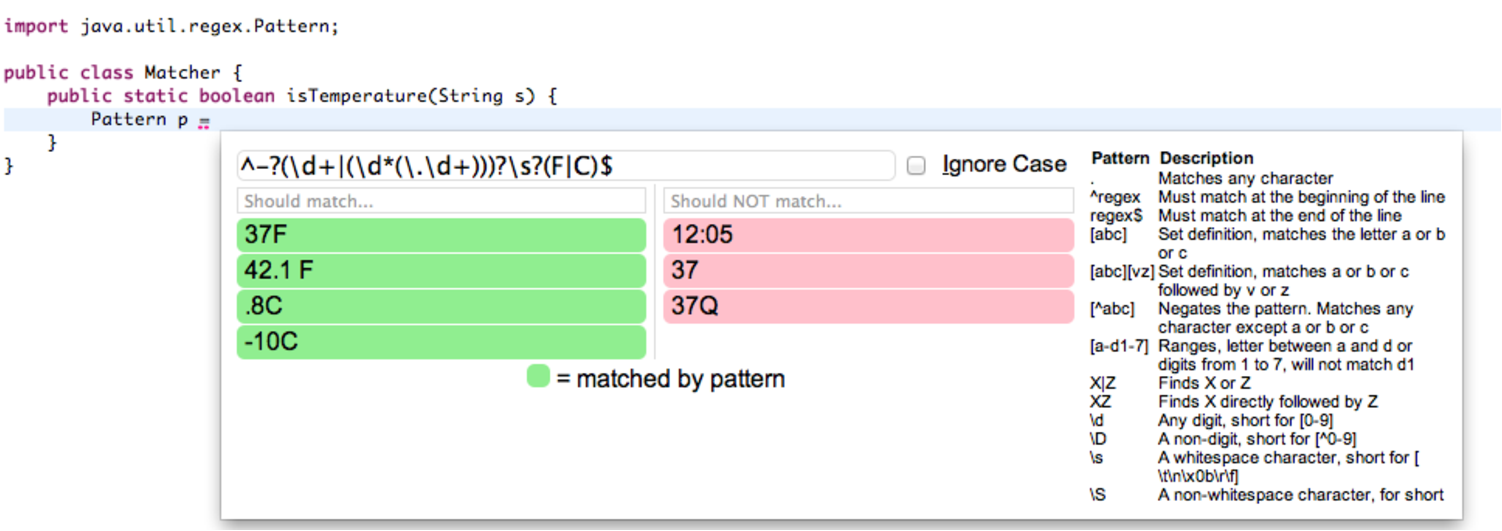
\includegraphics[scale=.55]{regex-palette.pdf}\\
$\Downarrow$ \text{(pressing \textbf{Enter})}\\
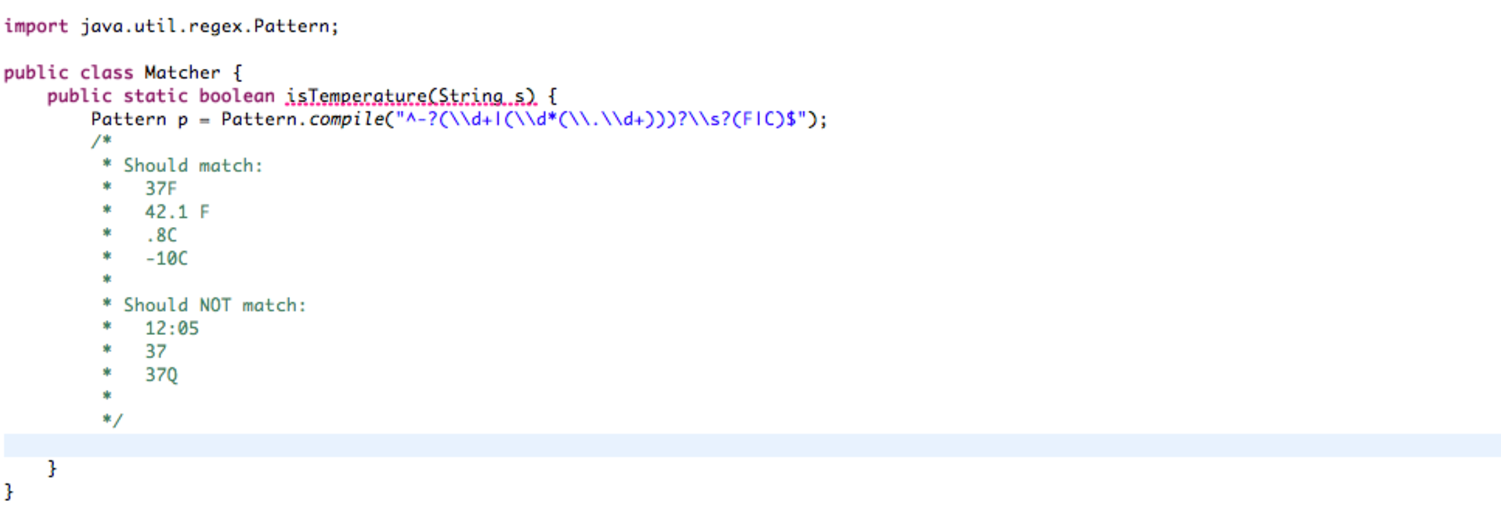
\includegraphics[scale=.55]{regex-code-generated.pdf}
\end{center}
\vspace{-20px}
\caption{An example of type-specific editor services, here shown for Java.}
\label{fig:regex-palette}
%\vspace{-10px}
\end{figure}

%In a conventional \emph{monolithic} programming system, support for each of these features would need to be built into the language and tools. 
No system today provides built-in support for all of the features enumerated above in their strongest form, so library providers must leverage  general-purpose mechanisms. %Unfortunately, it is impossible to completely define the syntax and the semantics referenced above using contemporary mechanisms, so library providers need to compromise. 
The most common strategy, exemplified by Java, is to ask clients to introduce patterns as strings, deferring their  parsing and compilation to run-time. This provides only a partial approximation to feature 1 due to clashes between string escape sequences and pattern escape sequences, as can be seen in the generated code at the bottom of Figure \ref{fig:regex-palette} (double backslashes are needed). Parsing errors due to these clashes have been observed to be difficult for even experienced programmers to diagnose \cite{Omar:2012:ACC:2337223.2337324}. Moreover, the static guarantees cannot be provided, leading to run-time exceptions (common even in well-tested code using regular expressions \cite{spishak2012type}), and mistakes that are not caught even at run-time, some of which can lead to security vulnerabilities due to injection attacks \cite{owasp2013}. It also introduces performance overhead due to run-time parsing and compilation of patterns, and redundant well-formedness checks.  

%Staging these computations can shift some of the errors and cost to compile-time, albeit with some additional semantic and syntactic complexity, but the issues related to the fact that a regular expression is not a string (e.g. syntactic clashes and injection attacks) persist.% parsing can move some errors to run-time, albeit at additional syntactic cost, but it also does not straightforwardly handle splicing-related issues, as we will discuss later.

A more semantically justifiable approach is to dispense with string representations entirely and directly work with an encoding of regular expression patterns using  general-purpose constructs like recursive sums and  products (e.g. as exposed by  datatypes in a functional language, shown in Sec. \ref{sec:syntax}, or a class hierarchy in an object-oriented language), or using an abstract data type. This provides feature 2a while sacrificing feature 1 (such an encoding affords only an approximation of the verbose abstract syntax of patterns, not their concrete syntax). Advanced invariants like those described in features 2b are not directly tracked by such encodings and require solutions beyond those commonly found in simply-typed languages (a feature like GADTs might suffice in this case \cite{XiCheChe03}).%Explicitly constructing a regular expression by applying datatype constructors is unacceptably verbose. 

None of these approaches address the important issue of tool support (feature 3). A number of tools are available online that provide services ranging from simple syntax highlighting to interactive testing and explanations of complex patterns \cite{regexr} and pattern extraction from examples (e.g. \cite{_txt2re:_????}). We have found that programmers benefit substantially from their use \cite{Omar:2012:ACC:2337223.2337324}. Unfortunately, evidence suggests that tools that must be accessed externally are difficult to discover and are thus used infrequently \cite{Murphy-Hill:2011:PIE:1958824.1958888,Campbell:2008:DRT:1636642.1636651,Omar:2012:ACC:2337223.2337324}. We have found that they are also less usable than editor-integrated tools %(e.g. \cite{IntelliJRegexp}) 
because they require the programmer to switch contexts and cannot make use of the code context \cite{Omar:2012:ACC:2337223.2337324}. %Working with high-level abstractions like these in a ``low-level'' editor is thus awkward and error-prone, just like attempting to work with high-level abstractions directly in terms of an encoding. 
For these reasons,   we see editor services as within the broad scope of an abstraction specification.

\subsubsection{Example 2: Regular Strings}\label{sec:rstr}
The examples above all dealt with how regular expression patterns are represented. However, programmers also want to reason about which regular language a string value is in \cite{sanitation-psp14}. For example, we might want to ensure that the arguments to a function called \verb|connect| corresponding to a database username and password are only alphanumeric strings. We might include this information directly in the type of \verb|connect|, i.e.
\begin{lstlisting}[numbers=none]
type alphanumeric = rstring[<SURL[A-Za-z0-9]+EURL>]
val connect : (alphanumeric * alphanumeric) -> DBConnection
\end{lstlisting}

This example uses a specialized \emph{type constructor}, \verb|rstring|, indexed by a statically known regular expression. The operations on such \emph{regular strings} would need a static semantics that track the regular language a string is in. For example, a regular string introduced by concatenating two other alphanumeric strings  should also be an alphanumeric string.

Ideally, we would be able to use standard string literal syntax with regular strings, e.g. 
\begin{lstlisting}[numbers=none]
let connection = connect("admin", "password")
\end{lstlisting}

Regular strings could go beyond simply refining standard string types. For example, they might define operators specific to regular strings like \emph{captured group projection}:
\begin{lstlisting}[numbers=none]
let example : rstring[<SURL(\d\d\d)-(\d\d\d\d)EURL>] = "555-5555"
let group0 (* : rstring[<\d\d\d>] *) = example#0
\end{lstlisting}
Ideally, it would be possible to define this operator such that its cost is $\mathcal{O}(1)$. %This example requires introducing new operators into the system that did not already exist, and using an underlying represention that differs for different type indices. 

\subsubsection{Example 3: Labeled Products with Functional Update Operators}\label{sec:lprod}
The simplest semantics for product types is to define only nullary and binary products \cite{pfpl}. However, in practice, many variations on product types are built in to various dialects of ML and other languages: $n$-ary tuples, labeled tuples, 
records (identified up to reordering), and 
records with width and depth coercions \cite{Cardelli:1984:SMI:1096.1098} and functional update operators \cite{ocaml-manual}. {The Haskell wiki notes that ''No, extensible records [i.e. records with a functional update operator] are not implemented in GHC. The problem is that the record design space is large, and seems to lack local optima. [...] As a result, nothing much happens.'' \cite{GHCFAQ}}%, 
 %mutable fields \cite{ocaml-manual}, 
%field delegation \cite{atlang-gpce14} \todo{gpce submission} 
%and 
% ``methods'' (i.e. pure objects) \cite{TSLs}


We would ideally like to avoid needing the language designer to decide \emph{a priori} on just one point in this large design space. Instead, they should simply provide some minimal way of defining products, perhaps only nullary and binary products, while making it possible for these other variations on products to be defined as libraries and used together without conflict. For example, we would like to be able to define labeled product types, which are like record types but maintain a row ordering. An example of a labeled product types classifying conference papers might be:
\begin{lstlisting}[numbers=none]
type Paper = lprod[{
  title : rstring[<SURL.+EURL>], 
   conf : rstring[<SURL[A-Z]+ \d\d\d\dEURL>]
}]
\end{lstlisting}

Because of the row ordering, it should be possible to introduce values of this type with or without explicit labels, e.g.
\begin{lstlisting}[numbers=none]
fun make_paper(t : rstring[<SURL.+EURL>]) : Paper = {title=t, conf="EXMPL 2015"}
\end{lstlisting}
should be equivalent to
\begin{lstlisting}[numbers=none]
fun make_paper(t : rstring[<SURL.+EURL>]) : Paper = (t, "EXMPL 2015")
\end{lstlisting}
Note above that we aim to be able to re-use the standard record and tuple syntax.

We should then be able to project out rows by providing a label (or a numeric index, not shown):
\begin{lstlisting}[numbers=none]
let test_paper = make_paper "Test Paper"
test_paper#conf
\end{lstlisting}

We might also be wish to support functional update. For example, an operation that dropped a row might be used like this:
\begin{lstlisting}[numbers=none]
let title_only (* : lprod[{title : rstring[<.+>]}] *) = test_paper.drop[conf]
\end{lstlisting}
An operation that added a row, or updated the value of an existing row, might be used like this:
\begin{lstlisting}[numbers=none]
fun with_author(p : Paper, a : rstring[<.+>]) = p.ext(author=a)
\end{lstlisting}
\subsection{Language-External Approaches}\label{external-approaches}


In situations, like these, where a library-based approach is not satisfying, providers must today take a \emph{language-external approach}, either by specifying a new system dialect (implementing it using a \emph{compiler generator} \cite{brooker1963compiler}, \emph{language workbench} \cite{erdweg2013state}, \emph{DSL framework} \cite{fowler2010domain}, or simply by forking an existing codebase), or by using an extension mechanism for a {particular} compiler\footnote{Compilers that modify, or allow modification of, the semantics of their base language, rather than simply permitting semantics-preserving optimizations, should be considered a pernicious means for creating new language dialects. That is, some programs that purport to be written in C, Haskell or Standard ML are actually written in compiler-specific dialects of these languages.}, editor or other tool. For example, a researcher interested in providing the regular expression related features just described (let us refer to these collectively as \texttt{R}) might design a new system with built-in support for them, perhaps basing it on an existing system containing some general-purpose features (\texttt{G}). A different researcher developing a new language-integrated parallel programming abstraction (\texttt{P}) might  take the same approach. A third researcher, developing a type system for reasoning about units of measure (\texttt{Q}) might again do the same. This results in a collection of distinct programming systems, as diagrammed in Figure \ref{approaches}a. 

Although often justified as ``proofs of concept'', this is a rather weak notion because no abstraction will be used entirely in isolation and such a construction gives us no rigorously justifiable  reason to believe that it can safely and naturally coexist with others specified or implemented in the same way. That is, one must either use the system containing features \texttt{G+R}, \texttt{G+P} or \texttt{G+Q}. There is no system containing \texttt{G}, \texttt{R}, \texttt{P} and \texttt{Q} in other combinations, and merging the systems containing each separately can be non-trivial because there can be serious interference and safety issues, as we will discuss at length throughout this thesis.
% More specifically, there is no guarantee of \textbf{orthogonality} or even \textbf{interoperability}.% This has limited the broad adoption of these kinds of innovations.%This latter method couples the semantics of the feature to the implementation details of a particular tool. Because the use of one implementation entails a different semantics for the feature than another, the extended tool acts, \emph{de facto}, as a distinct system for our purposes. 

%\paragraph{Orthogonality} Features implemented by language-external means like these cannot be adopted individually, but instead are only available coupled to a fixed collection of other features. This makes adoption more costly when these incidental features are  not desirable or are insufficiently developed (``toy languages''), or when the features bundled with a different language or tool are simultaneously desirable. 

Recent evidence indicates that this is one of the major barriers preventing research  from being driven into practice. For example, developers prefer high-level language-integrated parallel programming abstractions that provide  stronger semantic guarantees  \cite{cave2010comparing}, but library-based approximations are far more widely adopted because  ``parallel programming languages'' privilege only a few  abstractions at the language level. In contrast, it is widely acknowledged that  different abstractions are more appropriate in different situations \cite{Tasharofi:2013rc}. Moreover,  parallel programming is rarely the only relevant concern outside of a classroom or research setting. Support for regular expressions as above would be simultaneously desirable for processing large amounts of genomic data.% but using these features together in the same compilation unit would be difficult or impossible if implemented using language-external means. Indeed, switching to a ``parallel programming language'' would likely make it \emph{more} difficult to use regular expressions, as these are likely to be less well-developed in a specialized language than in an established general-purpose language.% This intuition was perhaps most succinctly expressed by a participant in a recent study by Basili et al. \cite{basili2008understanding}:  ``I hate MPI, I hate C++. [But] if I had to choose again, I would probably choose the same.'' %Similarly, a language and tools designed primarily to support regular expressions might make an interesting research project, but it would not be a suitable tool for writing large applications with more varied needs.

%\item Developing a new language and its associated tools places a significant development burden on providers who may wish only to promote a few core innovations, although tools like compiler generators, language workbenches and easy-to-extend tools can decrease this burden. 
%\item 

%Clients seem to prioritize the ability to choose different features for different portions of an application. 
%If calling between languages were safe and easy, then using a variety of specialized languages and associated tools might be less problematic. In fact, s
%Recognizing the limitations of relying on monolithic collection of primitives, some researchers have advocated instead for a model where multiple languages used within a single application, calling it the \emph{language-oriented approach} to software development \cite{languageoriented}. 

% \paragraph{Interoperability} Even in cases where, for each component of a software system, a programming system considered entirely satisfactory by its developers is available (e.g. a team goes through the trouble of implementing \verb|G+R+P| by reading papers about \verb|G+R| and \verb|G+P| and disentangling orthogonality-related issues), there remains a problem at any interface between  components written using a different combination of features. An interface that  externally exposes a specialized construct particular to one language (e.g. a function that requires a quantity having a particular unit of measure) cannot necessarily be safely and naturally consumed from another language (e.g. a parallel programming language). Tool support is also lost when calling into different languages. %We call this the \emph{interoperability problem}. % programs written by clients of a certain collection of features cannot always interface with programs written by clients of other features  in a safe, performant and natural manner.

% One strategy taken by proponents of a {language-oriented approach} \cite{journals/stp/Ward94} to partially address the interoperability problem is to  target an established intermediate language and use its constructs as a common language for communication between components written in different languages. Scala \cite{200464/IC} and F\# \cite{pickering2007foundations} are examples of prominent general-purpose languages that have taken this approach, and most DSL frameworks also rely on this strategy. As indicated in Figure \ref{approaches}a, this only enables interoperability in one direction. Calling into the common language becomes straightforward and safe, but calling in the other direction, or between the languages sharing the common target, does not, unless these languages are only trivially different from the common language. 

% %This approach only works well when new languages consist of constructs that can also be expressed safely and almost as naturally in the common language.
% %But many of the most innovative constructs found in modern languages (often, those that justify their creation) are difficult to define in terms of existing constructs in ways that guarantee all necessary invariants are statically maintained and that do not require large amounts boilerplate code and run-time overhead. 
% As a simple example with significant contemporary implications, F\#'s type system does not admit \verb|null| as a value for any type both defined and used within F\# code, but maintaining this sensible internal invariant still requires dynamic  checks because the stricter typing rules of F\# do not apply when F\# data structures are constructed by other languages on the Common Language Infrastructure (CLI) like C\# or SML.NET. This is not an issue exclusive to intermediate languages that make regrettable choices regarding \verb|null|, however. The F\# type system also includes support for checking that units of measure are used correctly \cite{syme2012expert, kennedy1994dimension}, but this more specialized static invariant is left entirely unchecked at language boundaries. Indeed, guidelines for F\# suggest that exposing functions that operate over values having units of measure, datatypes or tuples is not recommended when a component ``might be used'' from another language \cite{syme2012expert} because it is awkward to construct and consume these from other languages without the convenient primitive operations (e.g. pattern matching) and syntax that F\# includes. SML.NET prohibits exposing such types at component boundaries altogether. Moreover, it also cannot naturally consume F\# data structures, despite having a rather similar syntax and semantics in most ways (both languages directly descend from ML). 
%In Scala, traits that have default method implementations are difficult to implement from Java or other JVM languages and the workaround can break if the trait is modified \cite{scalatraitinterop}. 
%In some cases, desirable features must be omitted entirely due to concerns about interoperability. F\#, for example, aimed to retain source compatibility with Ocaml code, but due to the need for bidirectional interoperability with CLI languages, it does not support features like polymorphic variants, modules or functors \cite{ocaml-manual} because they have no apparent analogs in the type system of the CLI.
%\end{itemize}

\subsection{Language-Integrated Approaches}\label{language-integrated-approaches}
\begin{figure}
\begin{center}
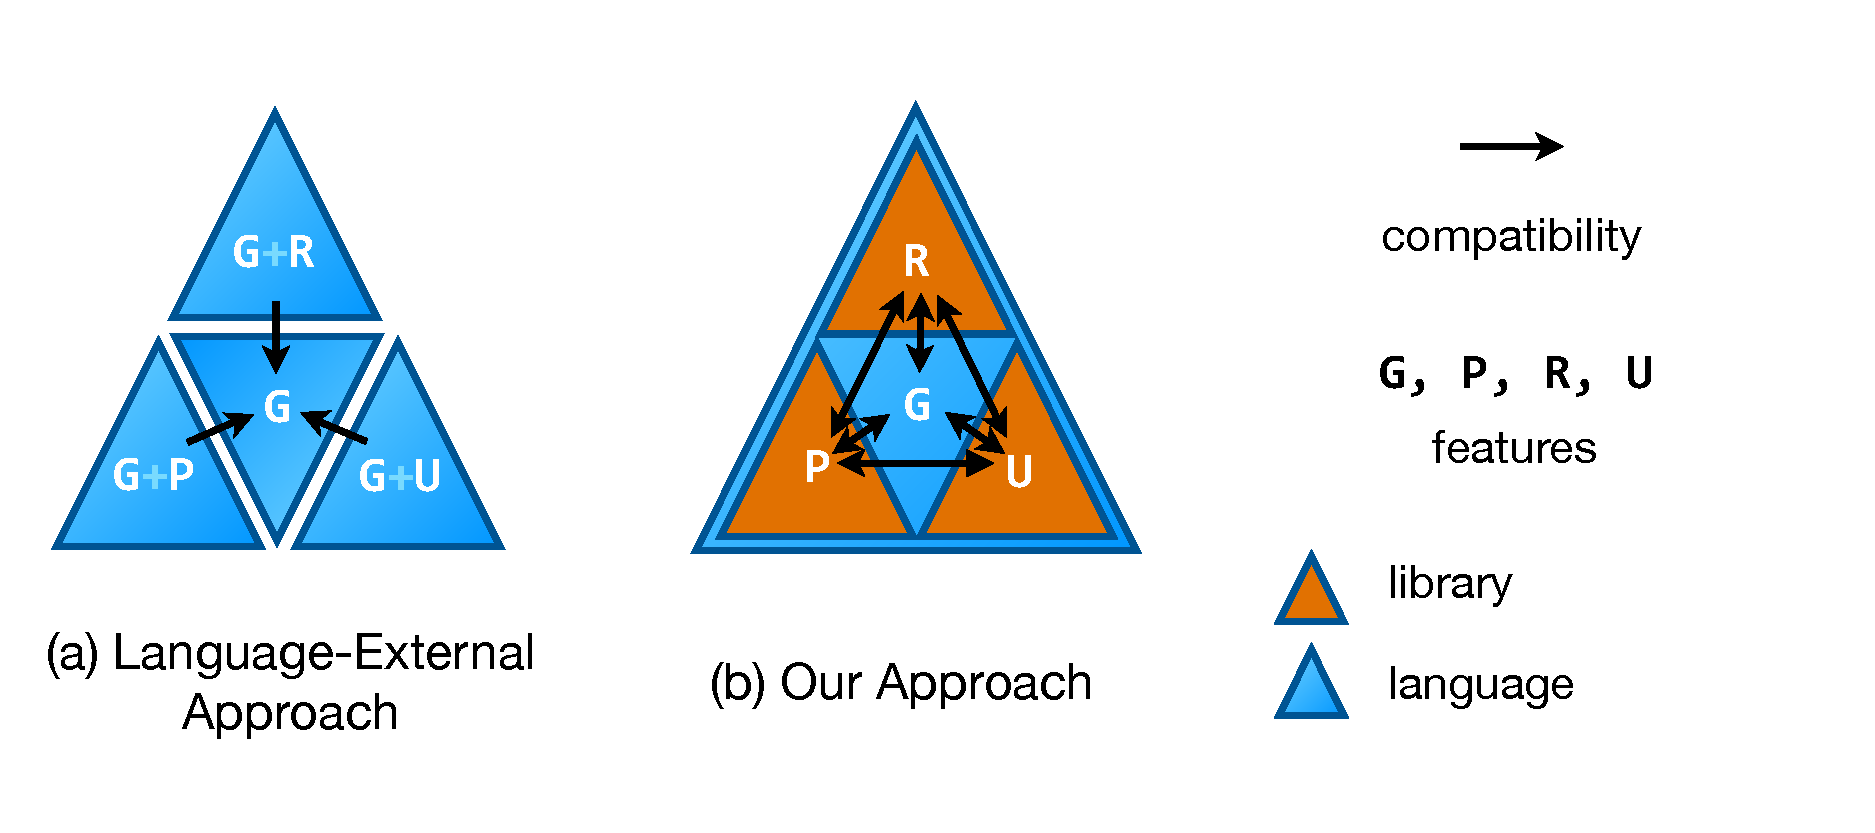
\includegraphics[scale=.48]{approaches.pdf}
\end{center}
\vspace{-20px}
\caption{\small (a) When taking a language-external approach, new features are packaged together into separate languages and tools. (b) When taking a language-integrated approach, there is one extensible host language and the compile-time and edit-time logic governing new constructs is expressed within ``active libraries''.}
\label{approaches}
%\vspace{-10px}
\end{figure}
We argue that, due to these problems, taking a language-external approach to realizing a new feature should be considered harmful and avoided whenever possible. The goal of the research being proposed here is to design \emph{language-integrated extension mechanisms} that give providers the ability to define, within libraries, new features that, like those above, that have previously required central planning, 
%\footnote{One might compare today's programming systems to  {centrally-planned} economies, whereas extensible\- systems more closely resemble modern market economies. Our safety constraints serve a role analagous to market regulation. We leave further development of this analogy to the reader.}
so that language-external approaches are less frequently necessary, as illustrated in Figure \ref{approaches}b. 
Such libraries have been called \emph{active libraries}  \cite{activelibraries} in that they more actively influence the syntax and semantics of the system. %Features implemented within active libraries can be imported individually, unlike features implemented by external means, giving us a potential means to avoid the problems of orthogonality and interoperability just described.

We must proceed with caution, however: critical issues having to do with {safety} must be overcome before language-integrated extension mechanisms can be introduced into a system. If too much control over  these core features of the system is given  to developers, the system may become quite unreliable. 
%For example, an extension could weaken important metatheoretic guarantees previously provided by the system. 
Type safety, for example, may not hold if the static and dynamic semantics of the language can be modified or extended arbitrarily from within libraries. Furthermore, even if extensions can be shown not to cause such problems in isolation, there may still be conflicts between extensions that could weaken their semantics, leading to subtle problems that only appear when two extensions are used together, thwarting any attempts to reason modularly about particular programs and the system as a whole. %As a simple example, if two active libraries introduce the same syntactic form but back it with differing (but individually valid) semantics, this ambiguity  would only manifest itself when both libraries were imported within the same scope. %Resolving these kinds of ambiguities requires significantly more expertise with parser technology than using the syntax itself does. 
These issues have plagued previous attempts to design language-integrated extensibility mechanisms.\todo{I can include a more detailed related work section if requested.}% We will briefly review some of these attempts below, then return to our approach.% To prevent them, our mechanisms will organize  extension logic around types to guarantee that extensions are both safe in isolation and also safely composable in any combination. 


 %This represents a minimalist approach to system design -- the conventional distinction between built-in and user-defined constructs is blurred and most features of the system are orthogonally implemented as {libraries}, rather than by the maintainers of the system.

%The mechanisms we describe will do so primarily by delimiting the scope of an extension to expressions of a single user-defined type or family of types. 

%This can be thought of as a more pernicious form of the conflict that arises when two globally-accessible constructs are given the same name. n languages without universal namespacing mechanisms (e.g. C, JavaScript, \LaTeX, ML and many others). 

%The extension mechanism\todo{elaborate on safety requirements + tension between expressiveness and safety, merge with next paragraph}. must be expressive enough to allow users to associate rich run-time, compile-time and edit-time behaviors with user constructs directly, while being sufficiently restrictive to maintain the global safety properties of the language and system as a whole, and to ensure that constructs cannot interfere with one another. 
